\documentclass[a4paper]{article}
\usepackage{xeCJK}
\setCJKmainfont[BoldFont=Heiti SC, ItalicFont=STSong]{Songti SC}
\setCJKsansfont[BoldFont=STHeiti]{STXihei}
\setCJKmonofont{STFangsong}
\usepackage{amsmath}
\usepackage{amsfonts}
\usepackage{geometry}
\usepackage{float}
\usepackage{graphicx}
\usepackage{enumitem}
\usepackage{pifont}
\usepackage[colorlinks]{hyperref}
\hypersetup{citecolor=DeepPink4}
\hypersetup{linkcolor=DarkRed}
\hypersetup{urlcolor=DarkBlue}
\usepackage{cleveref}
\geometry{a4paper,left=3cm,right=3cm,top=2cm,bottom=2cm}
\author{徐志鹏 517021910601}
\date{\today}
\title{信息安全数学基础大作业:\\RSA公钥密码系统的实现}
\begin{document}
\maketitle
\section{作业要求}
编程实现RSA密码系统:
\begin{enumerate}
    \item 随机产生大素数$p, q$(位长14-bit)以及$p\cdot q=n$.
    \item 随机产生公私钥对$(e, n)$及$d$.
    \item 对消息“m = Mathematical Fundation of Information security + 201904051 + 学号”进行数字化
    \item 对消息m加密和解密
\end{enumerate}
\section{文件说明}
我一共使用Python语言编写了7个文件,其相关功能说明如下:
\begin{itemize}
    \item[\checkmark] \textbf{Eratoshenes.py} - 使用平凡除法/厄拉托塞斯筛法计算小于10000的1229个素数,计算结果放入{Prime.py}文件中以供后续使用。
    \item[\checkmark] \textbf{fast\_power.py} - 模重复平方计算法,用以快速计算形如$b^n\ (mod\ m)$的算式。
    \item[\checkmark] \textbf{FermatTest.py} - 费马素性检验,用以检验随机生成的奇数是否是一个伪素数。 
    \item[\checkmark] \textbf{Prime.py} - 保存了小于10000的1229个素数。
    \item[\checkmark] \textbf{RandBigPrime.py} - 随机产生大素数
    \item[\checkmark] \textbf{rsa.py} - 主程序,完成消息输入,参数计算,加密解密的功能。
    \item[\checkmark] \textbf{str\_rsa.py} - 完成字符串的十六进制ASCII表示与整数之间格式的转换。
\end{itemize}
\section{运行}
\subsection{程序依赖}
\begin{itemize}
    \item 需要Python3.x版本,Python2.x版本无法正常运行。
    \item 需要且只需要Python的一个标准库random库用以生成随机整数。
\end{itemize}
\subsection{样例结果}
\begin{figure}[H]
    \centering
    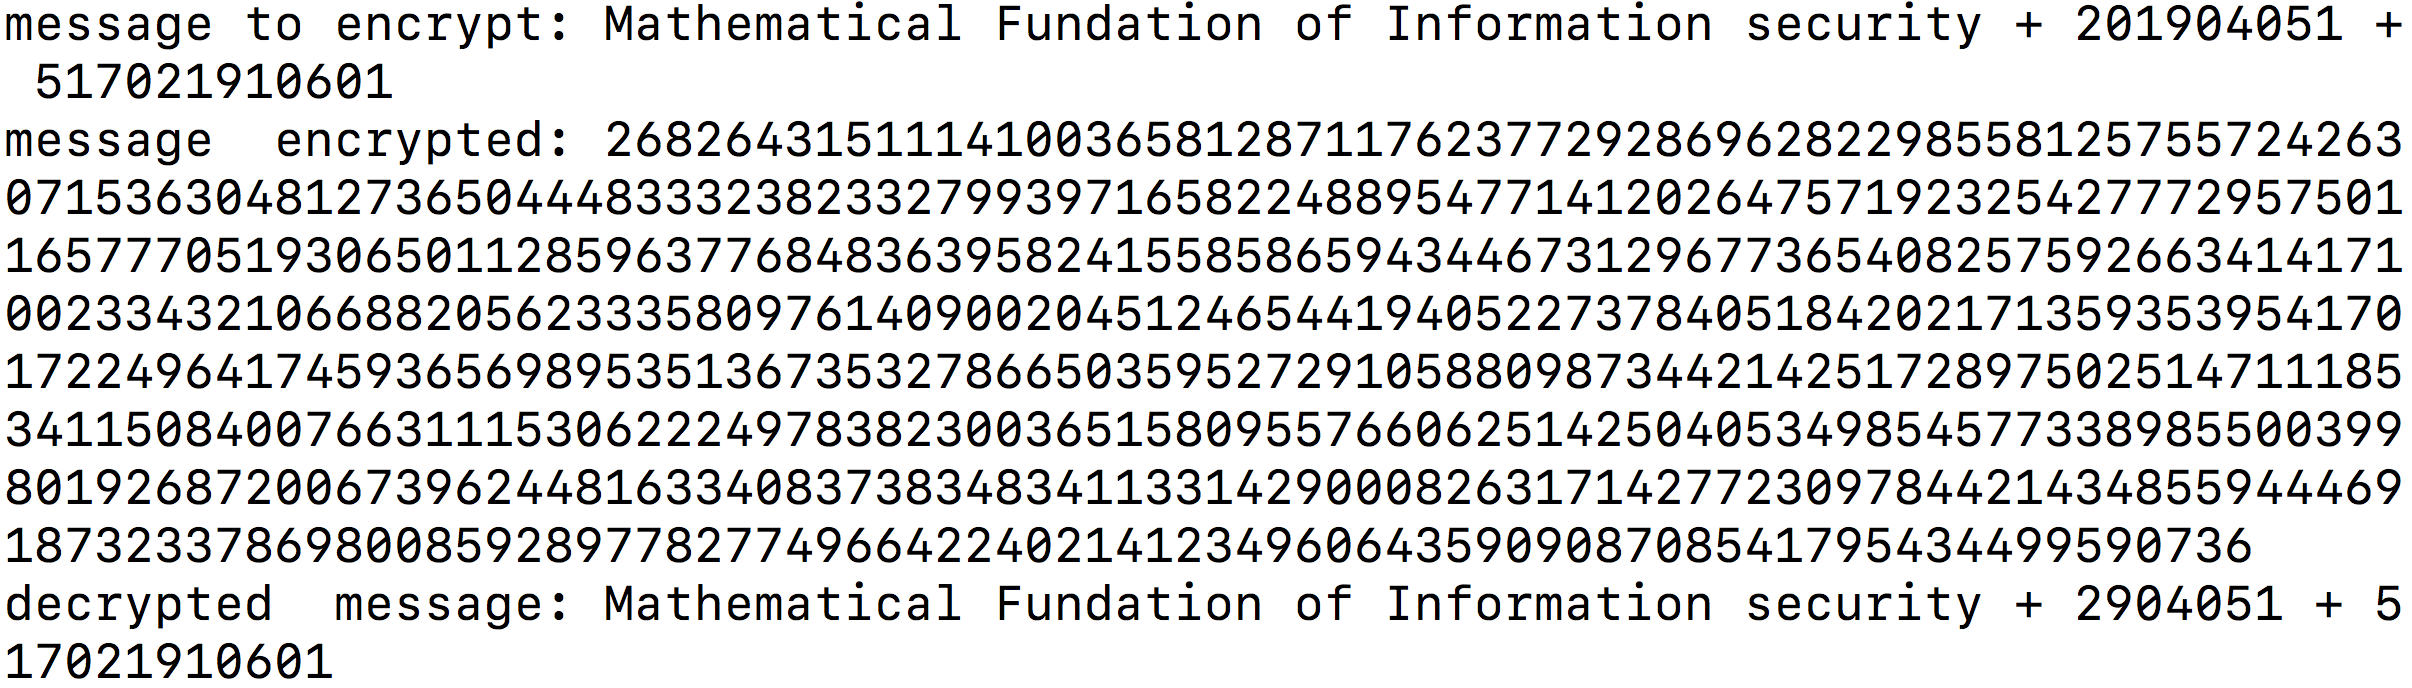
\includegraphics[width=.8\textwidth]{sample.png}
    \caption{样例输出}
    \label{fig:sample}
\end{figure}
\section{总体思路}
\subsection{产生大素数的思路}
首先用系统随机函数产生一个随机整数,若为偶数则加一成为奇数,然后使用10000内的素数试除,确定不存在小于10000的因子后进行费马素性检验,在多轮费马素性检验且成功之后可以假设该伪素数即为素数。
\subsection{加密思路}
由于每个字符可以转换为其对应的ascii码表示,所以将用户输入的一个字符串作为整体看作是一个大整数。

\section{具体实现步骤}
从程序功能从基本到全局的角度来说:
\begin{itemize}[label=\ding{212}]
    \item 首先,使用厄拉托塞斯筛法打表计算小于10000的1229个素数,计算结果会存储起来以供后续使用。
    \item 实现模重复平方计算功能。
    \item 实现大整数随机生成。每一位都随机从$0$到$F$中选择以生成十六进制格式的整数。
    \item 实现费马素性检验以判断任何给定的素数是否是伪素数。
    \item p,q全部按照RSA-1024标准采用了1028-bit长的格式,这样可以加密较长的字符串。
    \item 实现计算逆元的功能,用到了Bezout定理。
    \item 考虑了待加密字符串长度过长的情况,若待加密的数字大于n,则只截取字符串前面的部分字节加密。
    \item 主文件:\textbf{rsa.py},先随机生成$p, q$,计算$n, \phi(n)$,再随机生成与$\phi(n)$互素的$e, \\e^{-1}=d\ (mod\ \phi(n))$。
    \item 加密:$ciphertext\equiv plaintext^e\pmod n$
    \item 解密:$plaintext\equiv ciphertext^d\pmod n$
    \end{itemize}
\section{参考}
\begin{itemize}
    \item RSA周边——大素数是怎样生成的\\\hyperref[wef]{https://bindog.github.io/blog/2014/07/19/how-to-generate-big-primes/}
    \item 使用python生成固定长度的随机字符串\\\hyperref[fwe]{https://www.oschina.net/code/snippet\_153443\_4752}
\end{itemize}
\end{document}